\chapter{Hľadanie nadslova}

Problém, ktorý riešime v tejto práci sa dá rozdeliť na tri základné úrovne podľa toho,
ako veľmi berieme do úvahy požadovanú funkcionalitu a povahu reálnych dát. Pôjde o:
\begin{enumerate}
    \item Hľadanie $k$-nadslova
    \item Indexovanie do $k$-nadslova
    \item Tolerancia chýb v dátach
\end{enumerate}
V tejto kapitole sa pozrieme na prvú z týchto úrovní, pozrieme sa na ťažkosť problému
a na spôsob, akým vieme $k$-nadslovo hľadať efektívne, pokiaľ sú splnené pre naše
použitie rozumné predpoklady.

Mohlo by sa zdať, že hľadanie $k$-nadslova je slabšou verziou problému hľadania
spoločného nadslova, keďže ľubovoľné nadslovo nejakej množiny reťazcov bude zároveň
$k$-nadslovom tejto množiny reťazcov a ľahko vidno, že naopak to neplatí.
Ukazuje sa však, že rovnako, ako problém hľadania najkratšieho nadslova, je aj
problém hľadania najkratšieho $k$-nadslova $\mathcal{NP}$-ťažký.

%##################################################################################
\section{$\mathcal{NP}$-ťažkosť problému}
%##################################################################################

Rozhodovacia verzia problému najkratšieho spoločného nadslova je pomocou redukcie
z problému Hamiltonovskej cesty v orientovanom grafe s obmedzením na stupne vrcholov
a následnej redukcie na tento pomocný problém z problému Hamiltonovskej cesty v jednoduchom
grafe, $\mathcal{NP}$-úplný, pokiaľ je splnená aspoň jedna z nasledujúcich podmienok \cite{superstring}:
\begin{itemize}
    \item Veľkosť abecedy, nad ktorou máme zadané slovo je neobmedzená
    \item Veľkosť abecedy je aspoň $2$ a existuje $h \ge 1$ také, že každý
          vstupný reťazec má dĺžku $\lceil h \cdot log_2 (S) \rceil$, kde $S$
          je celková dĺžka vstupných slov.
\end{itemize}

Pokiaľ by sme vedeli efektívne riešiť rozhodovací problém najkratšieho $k$-nadslova,
na vstupe s rovnako dlhými vstupnými reťazcami a $k$ rovným dĺžke týchto reťazcov by
bolo riešenie zhodné s riešením rozhodovacieho problému najkratšieho spoločného nadslova.
Preto ak by sme mali polynomiálny algoritmus, ktorý vie riešiť rozhodovací problém
najkratšieho $k$-nadslova, mali by sme zároveň polynomiálny algoritmus riešiaci problém
Hamiltonovskej cesty. Trieda takýchto vstupov spĺňa druhú zo spomenutých podmienok.

Z toho vyplýva $\mathcal{NP}$-ťažkosť rozhodovacieho problému
najkratšieho $k$-nadslova a tým pádom aj $\mathcal{NP}$-ťažkosť problému hľadania
najkratšieho $k$-nadslova.

%###############################################################################
\section{Abstrakcia}
%###############################################################################

Po zdôvodnení a dokázaní ťažkosti riešeného problému sa pozrieme na spôsob, akým ho budeme
riešiť. Ako prvé si objasníme abstrakciu problému, na ktorej postavíme celé riešenie.

Podobne ako pri dokazovaní ťažkosti problému si pomôžeme grafovou teóriou. Celú
sadu vstupných slov si budeme reprezentovať ako mierne upravený ohodnotený de Bruijnov graf stupňa $k - 1$ nad
abecedou $\{A, C, G, T\}$. Každej hrane symbolicky priradíme reťazec, ktorého dĺžka bude
vždy zároveň hodnotou hrany.
Naše riešenie, čiže nejaké spoločné $k$-nadslovo, budeme reprezentovať ako sled v tomto grafe.

Vrcholmi v tomto grafe budú všetky $(k - 1)$-tice písmen ktoré sa vyskytujú v aspoň jednom slove.
Z vrchola $\left(x_1 x_2 x_3 \ldots x_{k-1}\right)$ bude do vrchola $\left(x_2 x_3 \ldots x_k\right)$
viesť hrana, ktorú označíme ako \emph{nutnú},
práve vtedy, ak slovo $x_1 x_2 x_3 \ldots x_k$ je podslovom niektorého zo
vstupných slov. Každej \emph{nutnej} hrane priradíme jednoprvkový reťazec pozostávajúci z $x_k$, čiže
posledného znaku vo vrchole, do ktorého smeruje.

Môžeme si všimnúť, že v takomto grafe budú všetky $k$-tice písmen, ktoré sú
ako podslovo niektorého vstupného slova, reprezentované ako \emph{nutné} hrany. Ďalej
potrebujeme zaviesť pojem \emph{nepovinnej} hrany.

Ak z vrchola $S_1$ nevedie \emph{nutná} hrana do vrchola $S_2$, tak z vrchola
$S_1$ vedie do vrchola $S_2$ \emph{nepovinná} hrana. Pre zadefinovanie hodnoty
hrany a priradeného reťazca potrebujeme ešte jeden pojem.

\begin{defn}
Nech $s_1$ a $s_2$ sú reťazce znakov a nech $z$ je najdlhší reťazec taký, že
$$\exists x, y \in \{A, C, G, T\}^*: s_1 = xz \wedge s_2 = zy \wedge |x| \ge 1 $$
Potom prekryvom reťazca $s_1$ s reťazcom $s_2$ označíme reťazec $z$ a dokončením $s_1$ v $s_2$ označíme
taký reťazec $y$, ktorý spĺňa $s_2 = zy$.
\end{defn}

\emph{Nepovinnej} hrane z vrchola $S_1$ do vrchola $S_2$ priradíme dokončenie $S_1$ v
$S_2$. Pripomíname, že hodnotou tejto hrany bude dĺžka priradeného reťazca.
Takto skonštruovaný graf k množine vstupných slov $S$ budeme označovať ako
\textbf{\boldmath$k$-graf množiny \boldmath$S$}.

Kvôli časti o implementácii si zadefinujeme ešte pojem \emph{nutného podgrafu}.
Pod pojmom \emph{nutný podgraf} $k$-grafu množiny $S$ budeme rozumieť faktorový
podgraf $k$-grafu množiny $S$ obsahujúci iba nutné hrany.

Môžeme si všimnúť, že reťazec priradený každej \emph{nutnej} hrane vieme vyjadriť
presne rovnako, ako reťazec priradený každej \emph{nepovinnej} hrane. Ďalším pozorovaním,
ktoré sa nám bude hodiť najmä pri implementácii je, že reťazec priradený každej
hrane vieme vypočítať iba z označení jej koncových vrcholov. Posledné dôležité
pozorovanie je, že každá hrana má kladnú cenu.

Slovo prislúchajúce sledu v $k$-grafe množiny $S$ získame ako zreťazenie $zr$, kde $z$ je
označenie prvého vrchola sledu a $r$ sú pospájané reťazce priradené hranám v takom
poradí, v akom sa tieto hrany nachádzajú v slede.

Formálnejšie zapísané, nech $slovo(V)$ označuje reťazec dĺžky $k-1$, označenie vrchola
$V$ a $slovo(e)$ označuje reťazec priradený hrane $e$. Potom $slovo(w)$, slovo
prislúchajúce sledu $w = V_1 e_1 V_2 e_2 \ldots e_{n-1} V_n$ skonštruujeme nasledovne: 
$$slovo(w) = slovo(V) \cdot slovo(e1) \cdot slovo(e2) \cdots slovo(e_{n-1}).$$
Pre prázdny sled $w$ definujeme $slovo(w) = \varepsilon$, čiže prázdne slovo.

Z tejto konštrukcie vidíme, že dĺžku slova priradeného neprázdnemu sledu vieme
vypočítať ako $k-1 + \sum \limits_{i=1}^{n-1} cena(e_i)$

Sled v $k$-grafe množiny $S$ budeme volať \emph{korektný}, ak obsahuje všetky \emph{nutné} hrany.
Teraz si dokážeme, že slovo prislúchajúce \emph{korektnému} sledu v $k$-grafe množiny $S$ je
$k$-nadslovom množiny $S$. K tomu budeme potrebovať ešte jednu pomocnú lemu.

\begin{lema}
\label{vertex_end_lemma}
    Nech $V_1 e_1 V_2 e_2 \ldots e_{n-1} V_n$ je sled v $k$-grafe nejakej množiny $S$.
    Potom sa reťazec $r$ prislúchajúci tomuto sledu končí $(k-1)$-ticou znakov zhodnou
    s označením vrchola $V_n$.
\end{lema}

\begin{proof}
    Matematickou indukciou na $n$, dĺžku sledu.
   
    $1^0:$ Ak $n$ je rovné $1$, sled obsahuje iba jeden vrchol. Podľa konštrukcie slova
           priradeného sledu bude toto slovo totožné s označením prvého a zároveň aj
           posledného vrchola v slede.

    $2^0:$ Nech $w_1 = V_1 e_1 \ldots V_{j-1}$ a $w_2 = V_1 e_1 \ldots V_j$. Podľa konštrukcie slova $slovo(w_2)$ platí
           $$ slovo(w_2) = slovo(V_1) \cdot slovo(e_1) \cdots slovo(e_{j-1}) = slovo(w_1) \cdot slovo(e_{j-1})$$
           Ďalej potrebujeme rozobrať dva prípady:
           \begin{enumerate}
            \item Ak je hrana $e_{j-1}$ \emph{nutná}, tak platí
                  $$ \exists x_1, x_2 \ldots x_k \in \{A, C, G, T \}: V_{j-1} = (x_1, \ldots , x_{k-1}) \wedge V_j = (x_2, \ldots , x_k)$$
                  a podľa konštrukcie hrany a priradenia jej reťazca, $slovo(e_{j-1}) = x_n$.
                  Z indukčného predpokladu vyplýva, že $\exists q \in \{ A, C, G, T\}^*: slovo(w_1) = q \cdot x_1 \cdot x_2 \cdots x_{k-1}$. Keď to
                  spojíme dohromady, dostaneme
                  $$ slovo(w_2) = slovo(w_1) \cdot slovo(e_{j - 1}) = q \cdot x_1 \cdots x_{k - 1} \cdot slovo(e_{j - 1}) = $$
                  $$ = q \cdot x_1 \cdots x_{k - 1} \cdot x_k = q' \cdot x_2 \cdots x_k = q' \cdot slovo(V_j),$$
                  kde $q' = qx_1$.

            \item Ak je hrana $e_{j - 1}$ \emph{nepovinná}, tak z konštrukcie \emph{nepovinnej} hrany a jej priradeného reťazca
                  vyplýva:
                  $$ \exists x, y, z \in \{ A, C, G, T\}^* : slovo(V_{j - 1}) = xz \wedge slovo(V_{j}) = zy \wedge slovo(e_{j - 1}) = y.$$
                  Opäť z indukčného predpokladu vyplýva $ \exists q \in \{A, C, G, T\}^*: slovo(w_1) = q \cdot slovo(V_{j-1}) = q \cdot xz$.
                  Keď to poskladáme dohromady, dostaneme
                  $$ slovo(w_2) = slovo(w_1) \cdot slovo(e_{j - 1}) = q \cdot x \cdot z \cdot slovo(e_{j - 1}) = q \cdot x \cdot z \cdot y = $$
                  $$ = q \cdot x \cdot slovo(V_j).\qedhere$$

           \end{enumerate}
\end{proof}

\begin{veta}
    Nech $W$ je \emph{korektný} sled v $k$-grafe množiny $S$. Potom $slovo(W)$ je $k$-nadslovom množiny slov $S$.
\end{veta}

\begin{proof}
Vezmime si ľubovoľné slovo $w$ také, že $|w| = k$ a $w$ je podslovom nejakého slova z $S$. Nech $x_1, x_2, \cdots x_k$
sú znaky tohto slova v poradí. Potom sa v grafe vyskytujú vrcholy $V_1 = (x_1, x_2, \cdots, x_{k-1})$ a $V_2 = (x_2, x_3, \cdots x_k)$ také,
že z $V_1$ ide hrana $e$ do $V_2$ a $e$ je \emph{nutná}. Z toho vyplýva, že $W$ = $U_1 V_1 e V_2 U_2$, kde $U_1, U_2$ sú nejaké časti sledu.
Z predošlej lemy potom vyplýva, že $\exists q \in \{A,C,G,T \}^*: slovo(U_1 V_1) =  q \cdot x_1 \cdots x_{k - 1}$ a teda
$$slovo(W) = slovo(U_1 V_1 e V_2 U_2) = q \cdot x_1 \cdots x_{k - 1} \cdot slovo(e) \cdot slovo (V_2 U_2) = q \cdot w \cdot slovo(V_2 U_2).\qedhere$$
\end{proof}

Nakoniec si spomenieme ešte jednu peknú vlastnosť, ktorá sa nám bude hodiť neskôr.

\begin{lema}
\label{shortest_edge_lemma}
    Nech $U$ a $V$ sú vrcholmi $k$-grafu množiny $S$. Potom najkratší sled z $U$
    do $V$ obsahujúci aspoň jednu hranu má rovnakú cenu, ako hrana $e$ z vrchola $U$ do $V$.
\end{lema}

\begin{proof}
    Sporom. Nech $w := U e_1 U_1 e_2 \cdots e_n V$ je kratšia cesta. Z lemy \ref{vertex_end_lemma} vieme,
    že aj $slovo(U e V)$ aj $slovo(w)$ sa končia označením vrchola $V$, zároveň, keďže $w$ má
    menšiu cenu ako $e$, platí $|slovo(w)| < |slovo(U e V)|$. To je ale v spore s tým, že prekryv
    $U$ s $V$ je najdlhší možný, $slovo(w)$ nám dáva návod, ako zostrojiť kratší.
\end{proof}

%##################################################################################
\subsection{Vlastnosti abstrakcie}
%##################################################################################

Zatiaľčo každému korektnému sledu v abstrakcii prislúcha práve jedno $k$-nadslovo, nie
každé $k$-nadslovo vieme reprezentovať ako sled v našom grafe.

Vezmime si ako vstupné slová \verb_ACG_ a \verb_CGA_ a $k$ rovné trom. Graf prislúchajúci
takémuto vstupu je znázornený na obrázku \ref{obr:graf}.
V grafe máme tri vrcholy zodpovedajúce dvojiciam \verb_(AC)_, \verb_(CG)_ a
\verb_(GA)_. Hrany aj s označením, ktoré budeme používať ďalej: 
\begin{itemize}
    \item \emph{nutná} hrana $e_1$ z vrchola \verb_(AC)_ do \verb_(CG)_ s priradeným reťazcom \verb_G_,
    \item \emph{nutná} hrana $e_2$ z vrchola \verb_(CG)_ do \verb_(GA)_ s priradeným reťazcom \verb_A_,
    \item \emph{nepovinná} hrana $e_3$ z vrchola \verb_(AC)_ do \verb_(GA)_ s reťazcom \verb_GA_,
    \item \emph{nepovinná} hrana $e_4$ z vrchola \verb_(CG)_ do \verb_(AC)_ s reťazcom \verb_AC_,
    \item \emph{nepovinná} hrana $e_5$ z vrchola \verb_(GA)_ do \verb_(AC)_ s reťazcom \verb_C_,
    \item \emph{nepovinná} hrana $e_6$ z vrchola \verb_(GA)_ do \verb_(CG)_ s reťazcom \verb_CG_.
    \item \emph{nepovinná} hrana $e_7$ z vrchola \verb_(AC)_ do \verb_(AC)_ s reťazcom \verb_AC_,
    \item \emph{nepovinná} hrana $e_8$ z vrchola \verb_(CG)_ do \verb_(CG)_ s reťazcom \verb_CG_,
    \item \emph{nepovinná} hrana $e_9$ z vrchola \verb_(GA)_ do \verb_(GA)_ s reťazcom \verb_GA_.
\end{itemize}

\begin{figure}

\centerline{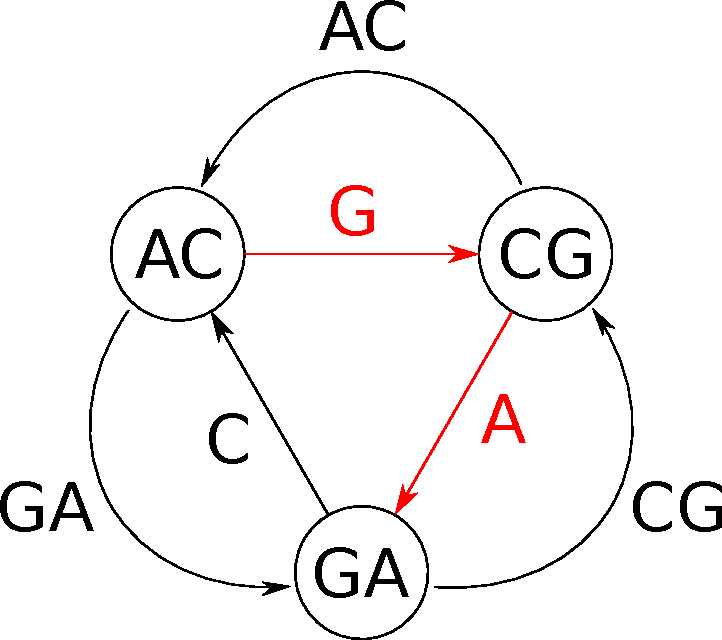
\includegraphics[width=0.5\textwidth]{images/graph-2-1-3.pdf}}

\caption[Príklad grafu]{Príklad $2$-grafu množiny $\{\texttt{ACG}, \texttt{CGA} \}$. \emph{Nutné} hrany sú vyznačené
červenou farbou, čierne hrany sú \emph{nepovinné}.}

\label{obr:graf}

\end{figure}

Celkom ľahko vidíme, že najkratšie možné $k$-nadslovo musí mať aspoň $4$ znaky. Vhodné $k$-nadslovo takejto
dĺžky naozaj existuje, napríklad \verb_ACGA_. V našom grafe ho vieme reprezentovať ako sled:
$$\texttt{(AC)} e_1 \texttt{(CG)} e_2 \texttt{(GA)}$$

Ak sa ale pozrieme napríklad na slovo \verb_TTACGTTTCGATT_, neexistuje žiaden sled, ktorému prislúcha toto $k$-nadslovo,
keďže žiaden vrchol ani hrana neobsahujú znak \verb_T_. Ľahko ale vidíme, že toto slovo vieme skrátiť
vynechaním znakov \verb_T_, ktoré sa nemôžu objaviť v žiadnom $k$-nadslove konštruovanom k sledu,
na stále vyhovujúce nadslovo \verb_ACGCGA_. Toto slovo vieme reprezentovať ako sled:
$$\texttt{(AC)} e_1 \texttt{(CG)} e_8 \texttt{(CG)} e_2 \texttt{(GA)}$$

Zdá sa teda, že ak nejakú časť $k$-nadslova nevieme reprezentovať ako časť sledu v $k$-grafe, môžeme ju
nejakým spôsobom vynechať. Túto vlastnosť si ďalej zhrnieme. Predtým si zadefinujeme konštrukciu sledu k
ľubovoľnému $k$-nadslovu.

\begin{defn}
    Nech $S$ je množina slov nad abecedou $\Sigma$, $s = x_1 x_2 \cdots x_n$ je nejakým slovom nad abecedou $\Sigma$,
    nech $G$ je $k$-grafom množiny $S$, nech \\
    $Z = \{ i \in \{1 \ldots n - k + 2 \} | (x_i x_{i+1} \cdots x_{i+k-2}) \in V(G) \}$, čiže množina takých indexov v $s$, že
    $k-1$-tica písmen začínajúca na tejto pozícii označuje vrchol v grafe $G$
    a nech $v_i$ je $i$-ty najmenší prvok množiny $Z$. Potom pre neprázdnu množinu $Z$ určíme \textit{$k$-sled slova $s$ pri množine $S$} ako
    $$sled_{k,S}(s) = V_1 e_1 V_2 e_2 \cdots e_{p-1} V_p,$$
    kde $V_i = (x_{v_i} x_{v_i + 1} \cdots x_{v_i + k - 2})$ a $e_i$ je hrana medzi $V_i$ a $V_{i+1}$. Pre prázdnu
    množinu $Z$ určíme $sled_{k, S}(s)$ ako prázdny sled.
\end{defn}

Na túto konštrukciu sa vieme pozerať aj tak, že zo slova $s$ vytiahne tie časti -- vrcholy, ktoré vieme reprezentovať
v našom grafe $G$ a pospája ich hranami. To, že táto konštrukcia zachytáva všetky pre nás dôležité časti slova
a zároveň ho nenafúkne, si ďalej dokážeme.

\begin{veta}
    Nech $s = x_1 x_2 \cdots x_n$ je $k$-nadslovom množiny $S$. Potom aj $slovo(sled_{k,S}(s))$ je
    $k$-nadslovom množiny $S$.
\end{veta}

\begin{proof}
    Nech $q = a_1 a_2 \cdots a_k$ je ľubovoľná $k$-tica písmen vyskytujúca sa v nejakom slove množiny $S$.
    Keďže $s$ je $k$-nadslovom množiny $S$, platí nasledovné: 
    $$\exists i : a_1 = x_i \wedge a_2 = x_{i+1} \wedge \ldots \wedge a_k = x_{i+k-1}$$
    Zároveň z konštrukcie $k$-grafu množiny $S$ vyplýva, že obsahuje vrcholy $U_1 := (x_i x_{i+1} \cdots x_{i+k-2})$
    a $U_2 := x_{i+1} x_{i+2} \cdots x_{i+k-1}$. Tým pádom množina $Z$ z konštrukcie sledu obsahuje aj $x_i$, aj
    $x_{i+1}$, čiže $sled_{k,S}(s)$ obsahuje podsled $U_1 e U_2$ a teda $slovo (sled_{k,S}(s))$ obsahuje $q$.
\end{proof}

\begin{veta}
    Nech $S$ je množina slov nad abecedou $\Sigma$, $n$ je prirodzené a $k \ge 2$ je celé číslo, nech $s = a_1 a_2 \cdots a_n$ je
    nejakým slovom nad $\Sigma$. Potom $|slovo(sled_{k,S}(s))| \leq |s|.$
\end{veta}

\begin{proof}
    Nech $G$ je $k$-graf množiny $S$. Dokážeme matematickou indukciou na $n$, dĺžku slova $s$.

    $1^0:$  $n < k-1$. Tento prípad pokrýva napríklad prázdne slová $s$, čiže je vhodný ako báza indukcie.
            
            V $s$ sa nenachádza žiadna $k-1$-tica písmen, čiže množina $Z$ z konštrukcie $k$-sledu bude prázdna, teda aj $sled_{k,S}(s)$ bude
            prázdny, čiže $slovo (sled_{k,S}(s)) = \varepsilon, |\varepsilon| = 0 \leq n$.

    $2^0:$  Položíme $s' := a_1 a_2 \cdots a_{n-1}$, čiže $s$ skrátený o posledný znak. 
            V indukčnom kroku nás zaujímajú iba slová $s$ dĺžky aspoň $k - 1$. Rozoberieme tri základné možnosti:
            \begin{itemize}
                \item $(a_{n-k+2} a_{n-k+3} \cdots a_n) \notin V(G).$ Množina $Z$ z konštrukcie sledu bude rovnaká
                      pre $s$ aj $s'$, čiže $slovo(sled_{k,S}(s)) = slovo (sled_{k,S}(s'))$ a teda \\ 
                      $|slovo(sled_{k,S}(s))| = |slovo(sled_{k,S}(s'))| \leq |s'| < |s|$, kde prvá nerovnosť vyplýva z indukčného predpokladu.
                \item $(a_{n-k+2} a_{n-k+3} \cdots a_n) \in V(G)$ a $sled_{k,S}(s')$ je prázdny. Potom množina $Z$ z konštrukcie
                      sledu k $s$ bude obsahovať jeden prvok, čiže $sled_{k,S}(s)$ obsahuje iba jeden vrchol. Preto $|slovo(sled_{k,S}(s))| = k - 1 \leq |s|$.
                \item $V_0 := (a_{n-k+2} a_{n-k+3} \cdots a_n) \in V(G)$ a $sled_{k,S}(s')$ je neprázdny. Položíme \\
                      $j := max \{ i \in \{1 \ldots n - k + 1 \} | (x_i x_{i+1} \cdots x_{i+k-2}) \in V(G) \}$,
                      čiže začiatok poslednej $k-1$-tice zodpovedajúcej nejakému vrchola v $G$ a $s'' := a_1 a_2 \cdots a_{j+k-2}$,
                      čiže $s'$ skrátené po koniec poslednej $k-1$-tice zodpovedajúcej nejakému vrchola v $G$. Slová $s'$ a $s''$ majú
                      rovnakú množinu $Z$ z konštrukcie sledu, čiže majú priradený rovnaký sled a teda $slovo(sled_{k,S}(s')) = slovo(sled_{k,S}(s''))$.

                      Položme $sled_{k,S}(s'') = V_1 e_1 \cdots V_p$. Sled k slovu $s$ obsahuje práve jeden vrchol navyše, čiže $sled_{k,S}(s) = V_1 e_1 \cdots V_p e_p V_0$,
                      kde $e_p$ je hrana z $V_p$ do $V_0$. Z konštrukcie slova k sledu vieme nasledovné: \\
                      $$slovo(sled_{k,S}(s)) = slovo(V_1) slovo(e_1) slovo(e_2) \cdots slovo(e_p) = $$
                      $$ = slovo(sled_{k,S}(s'')) \cdot slovo(e_p).$$
                        Podľa lemy \ref{vertex_end_lemma} sa $slovo(sled_{k,S}(s''))$ končí označením vrchola $V_q$, čiže rovnako, ako $s''$,
                      podobne sa $slovo(sled_{k,S}(s))$ končí tou istou $k-1$-ticou ako $s$, z indukčného predpokladu vyplýva, že $|slovo(sled_{k,S}(s''))| \leq |s''|$.
                      Ak by teda platilo $|slovo(sled_{k,S}(s))| > |s|$, bolo by dokončenie $s$ v $s''$ kratšie, než dokončenie $V_0$ vo $V_q$,
                      čo je v spore s tým, že prekryv $V_0$ s $V_q$ je definovaný ako najdlhší možný, podobne ako v dôkaze lemy \ref{shortest_edge_lemma}.
                      Aj v tomto prípade teda platí indukčný krok. \qedhere
            \end{itemize}
    
\end{proof}

\begin{dosl}
    Nejaké najkratšie $k$-nadslovo množiny $S$ zodpovedá nejakému najlacnejšiemu \emph{korektnému} sledu v $k$-grafe množiny $S$.
\end{dosl}

%##################################################################################
\section{Implementácia}
%##################################################################################

V predošlej časti sme si dokázali, že pre nájdenie najkratšieho $k$-nadslova množiny slov $S$
nám stačí nájsť najlacnejší korektný sled v $k$-grafe množiny $S$, čiže sled, ktorý obsahuje
všetky \emph{nutné} hrany grafu. Ide o pomerne známy \textbf{problém vidieckeho poštára} z grafovej teórie,
ktorý je vo všeobecnom prípade $\mathcal{NP}$-ťažký \cite{ruralpostman}.

Ukazuje sa však, že pokiaľ podgraf $k$-grafu množiny $S$ obsahujúci iba \emph{nutné} hrany je súvislý,
tento problém je polynomiálne riešiteľný a riešenie je takmer zhodné s riešením \textbf{problému čínskeho
poštára} na orientovaných grafoch. Keďže zamýšľané použitie $k$-nadslova je na reprezentáciu sekvenčných čítaní, ktoré sú
krátkymi podreťazcami celého genómu s vysokou mierou pokrytia, je pomerne pravdepodobné, že nutné hrany
$k$-grafu týchto čítaní budú tvoriť stále súvislý graf, prípadne že budú obsahovať iba málo komponentov.
Najprv sa teda pozrieme, ako hľadať $k$-nadslovo v súvislom $k$-grafe.

%##################################################################################
\subsection{Súvislý graf}
%##################################################################################

Problém čínskeho poštára sa zaoberá hľadaním najlacnejšieho sledu v grafe takého, že
každou hranou prejde aspoň raz.

Základnou myšlienkou riešenia problému čínskeho poštára je pridať hrany s čo najmenším súčtom do grafu
tak, aby obsahoval eulerovský ťah \cite{chinesepostman}. Tento prístup funguje preto, že každý sled priamo
zodpovedá eulerovskému ťahu pre nejaké doplnenie hrán do grafu.

Súvislý orientovaný graf obsahuje eulerovskú kružnicu práve vtedy, keď vstupný stupeň $\delta_I$ je rovný
výstupnému stupňu $\delta_O$ v každom vrchole, eulerovský ťah existuje aj v prípade, keď sa v najviac
dvoch vrcholoch vstupný a výstupný stupeň líšia o $1$. Ak teda $k$-graf množiny $S$ má túto
vlastnosť, nájdenie korektného sled je už len záležitosťou nájdenia eulerovského ťahu.

Pokiaľ nutný podgraf $k$-graf množiny $S$ túto vlastnosť nemá, potrebujeme čo najlacnejšie pridať hrany z vrcholov s 
$\delta_O < \delta_I$ do vrcholov s $\delta_I < \delta_O$, pričom využívať môžeme aj nepovinné hrany.
Z lemy \ref{shortest_edge_lemma} vyplýva, že najlacnejšia cesta medzi dvomi vrcholmi je hrana medzi
nimi, čiže zaujímať nás budú iba hrany medzi vrcholmi. Z toho vyplýva aj konštrukcia nasledovného grafu.

\begin{defn}
    Nech $G$ je $k$-graf množiny $S$ a $G'$ je jeho nutný podgraf. Tokovým grafom grafu $G$
    označíme graf $H$, ktorého množinu vrcholov skonštruujeme nasledovne:
    $V(G') = \{s, t\} \cup V_h \cup V_p$, kde $V_h$ (hladné) je množina $\{ v \in V(G) | \delta_O^{G'}(v) > delta_I^{G'}(v) \}$
    a $V_p$ (presýtené) je množina $\{ v \in V(G) | \delta_I^{G'}(v) > delta_O^{G'}(v)\}$.
    Hrany grafu $H$ budú troch typov:
    \begin{enumerate}
        \item Tie hrany z grafu $G$, ktoré idú z presýteného vrchola do hladného s cenou rovnakou ako v $G$ a kapacitou $\infty$,
        \item Hrany od $s$ do každého vrchola vo $V_p$ s cenou $0$. Kapacitu takéhoto typu hrany do vrchola $U$ určíme ako $\delta_I^{G'}(U) - \delta_O^{G'}(U)$,
        \item Hrany od každého vrchola z $V_h$ do $t$ s cenou $0$. Kapacitu takéhoto typu hrany z vrchola $U$ určíme ako $\delta_O^{G'}(U) - \delta_I^{G'}(U)$.
    \end{enumerate}
    Žiadne iné hrany v grafe $H$ nebudú.
\end{defn}

Nájdenie najlacnejšieho maximálneho toku v tokovom grafe $k$-grafu bude zodpovedať
najlacnejšiemu možnému pridaniu hrán do nutného podgrafu $k$-grafu tak, aby v ňom existovala eulerovská
kružnica. Jednoducho sa pre každý nasýtený vrchol $V$ a hladný vrchol $U$ pridáme $x$ hrán z $V$ do $U$,
kde $x$ je veľkosť toku tečúca z vrchola $V$ do $U$.

Keďže náš korektný sled nemusí začínať aj končiť v tom istom vrchole, potrebujeme
nájsť v skutočnosti najlacnejší tok, ktorý je o $1$ menší než maximálny a pridať hrany podľa neho.
Takýto tok môžeme nájsť napríklad pomocou algoritmu od Edmondsa a Karpa \cite{mincost_maxflow} v
čase $O(n^3)$ kde $n$ je počet vrcholov v tokovom grafe nášho $k$-grafu, prípadne pomocou akéhokoľvek potenciálne rýchlejšieho
algoritmu na $2$ simulácie, kde v tej druhej si vhodným pridaním jedného vrchola vieme vynútiť
obmedzenie najväčšieho toku na hodnotu o $1$ menšiu, než zistíme pri prvej simulácii.

Ako posledné nám teda stačí nájsť eulerovský ťah v takto upravenom grafe a zrekonštruovať z neho
nadslovo. Týmto sme si popísali polynomiálny algoritmus na hľadanie $k$-nadslova, pokiaľ je
nutný podgraf $k$-grafu súvislý. Pre rekapituláciu si celý algoritmus uvedieme v dôkaze nasledujúcej
vety.

\begin{veta}
    Nech $S$ je množina slov dlhých aspoň $k$ nad abecedou $\Sigma$. Potom ak je nutný podgraf $k$-grafu množiny $S$
    súvislý, existuje polynomiálny algoritmus na hľadanie $k$-nadslova.
\end{veta}

\begin{proof}
    Uvedieme si algoritmus, ktorý $k$-nadslovo nájde. Ku každému kroku uvedieme aj časovú zložitosť od počtu slov v
    množine $S$, pre jednoduchosť za predpokladu, že každý reťazec má rozumne malú fixnú dĺžku.
    \begin{enumerate}
        \item Zostav nutný podgraf $k$-grafu zo vstupných slov a prečísluj vrcholy do intervalu $\left[0, pocet\right)$. $O(nk)$
        \item Vyrieš problém najlacnejšieho maximálneho toku na tokovom grafe. $O(n^3)$
        \item Pridaj hrany do grafu podľa výsledného toku. $O(n^2)$
        \item Nájdi eulerovský ťah. $O(n)$
        \item Transformuj eulerovský ťah na $k$-nadslovo. $O(nk)$ \qedhere
    \end{enumerate}
\end{proof}

Poslednou vecou, ktorou sa budeme zaoberať v súvislom prípade, je časová zložitosť. Všetky časti
algoritmu sa vykonávaju v čase lineárne závislom od veľkosti vstupu, okrem druhého a tretieho bodu.
V týchto bodoch je pomerne nepravdepodobné, že existuje riešenie rýchlejšie, než kvadratické. To je
spôsobené tým, že v najhoršom prípade môžu takmer všetky vrcholy grafu mať $\delta_I$ rôzne od $\delta_O$
a algoritmus, ktorý nájde najlepšie priradenie, sa potrebuje pozrieť na každú hranu.

Keďže hľadanie
$k$-nadslova chceme využiť do dátovej štruktúry schopnej reprezentovať milióny až stovky miliónov
genetických čítaní, chceli by sme mať nejaký spôsob, ako v lineárnom čase nájsť aspoň nejaké rozumné
pospájanie týchto vrcholov. V našom navrhovanom riešení jednoducho vyskúšame pevne stanovený počet
náhodných priradení a vyberieme z nich to najlacnejšie.


